\documentclass[UTF8, 12pt]{ctexart}
\usepackage{enumitem}
\usepackage{amsmath}
\usepackage{amssymb}
\usepackage{amsfonts}
\usepackage{mathrsfs}
\usepackage{XCharter}
\usepackage{fancyhdr}
\setCJKmainfont{DENGL.TTF}
\usepackage{eulervm}
\usepackage{graphicx}

\topmargin -.5in
\textheight 9in
\oddsidemargin -.25in
\evensidemargin -.25in
\textwidth 7in
\pagestyle{fancy}

\newenvironment{proof}{\\\ignorespaces\textbf{Proof:}}{\hfill $\square$\par\noindent}
\newenvironment{solution}{\ignorespaces\textbf{Solution:}}{\hfill $\square$\par\noindent}

\newenvironment{rcases}{\left.\begin{aligned}}{\end{aligned}\right\rbrace}

\title{Fair Dice}
\author{张志成 518030910439}
\date{\today}

\begin{document}
    \maketitle

    \section{Problem}
    骰子的六个面上分别有数字1,...,6。假设你有办法对骰子内部添东西使得抛掷后各个面出现的概率分布为给定分布。是否可以造出两个骰子,同时抛出后得到的两个数
    之和在2,...,12之间等概率分布?

    \section{Solution}
    I utilize the tool of Generative Function to represent the distribution of each roll. 
    $$ P(x) = p_1x + p_2x^2 + p_3x^3 + p_4x^4 + p_5x^5 + p_6x^6 $$
    Here, $p_i$ represents the probability of the dice roll being $i$.
    
    With 2 dices, we can simply multiply two generative functions.
    \begin{align*}
        P(x) &= p_1x + p_2x^2 + p_3x^3 + p_4x^4 + p_5x^5 + p_6x^6 \\
        Q(x) &= q_1x + q_2x^2 + q_3x^3 + q_4x^4 + q_5x^5 + q_6x^6 \\
        \therefore T(x) &= P(x)Q(x) \\ &= (p_1x + p_2x^2 + p_3x^3 + p_4x^4 + p_5x^5 + p_6x^6)(q_1x + q_2x^2 + q_3x^3 + q_4x^4 + q_5x^5 + q_6x^6) \\
        &= t_2x^2 + ... + t_{12}x^{12}
    \end{align*}
    The problem asks for a equal distribution between 2 and 12.
    Thus, we have the following constraints:
    \begin{align}
        t_2 = t_3 = ... = t_{12} &= \frac{1}{11} \\
        \sum_{i = 1}^{6} p_i &= 1 \\
        \sum_{i = 1}^{6} q_i &= 1
    \end{align}
    The is a set of equations. So I tried using mathematica to solve it but it only yields complex number answers, which is not accpetable. Below is the code I use:
    \begin{figure}[htbp]
        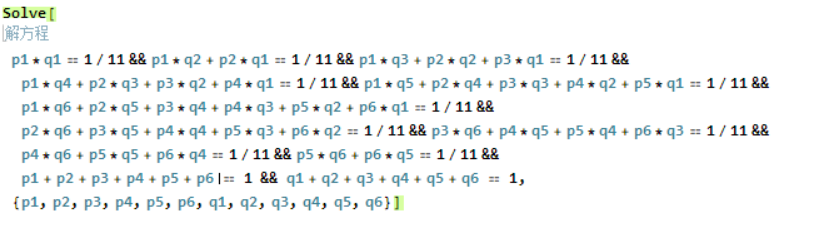
\includegraphics{solve.png}
        \caption{Mathematica sucks}
    \end{figure}

    So we have to further consider these constrains.
    \begin{align*}
        P(x)Q(x) &= \frac{1}{11} * (x^2 + ... + x^{12}) \\
        &= \frac{1}{11} * x^2 * \frac{x^{11}-1}{x-1}
    \end{align*}
    
    The problem is really asking if there are any factorization of $x^2 * \frac{x^{11}-1}{x-1} \in \mathbb{R}[x]$.

    But there is none since the only root $x \in \mathbb{R}$ is 1. This result is confirmed using Mathematica, see \textit{factor.png} in the folder.
    \section{Conclusion}
        I used the above method to show that no solution exists. Futher explorations still interest me whether there is a
        pattern of possible distribution feasible under this rule.
\end{document}